\chapter{Event reconstruction}

\intro{The reconstruction of basic analysis objects within an event is described. A key ingredient in the \gls{cms} reconstruction is the particle flow algorithm which defines particle candidates by combining various subdetector information. The focus is set on the reconstruction and performance of muons, electrons, jets, and the missing transverse energy in 8 and 13~TeV pp~collision data which are the input objects in this thesis to study single top quark production.}

The event reconstruction attempts to reconstruct and identify basic analysis objects from the raw detector data. In \gls{cms}, basic objects are particle tracks and vertices as well as charged lepton, photon, and jet candidates. During the reconstruction additional information such as the missing transverse energy, $\met$, and the likelihood of jets to originate from the hadronization of b~quarks~(``b-tagging'') is determined. Since $\tau$ leptons and photons are not relevant for the study of $t$-channel single top quark production a description of their reconstruction and performance is omitted here yet details can be found in Refs.~\cite{Khachatryan:2015iwa,Khachatryan:2015dfa}.


%##############################################
\section{Track and vertex reconstruction}
%##############################################

The track reconstruction is split in two steps. First, in the local reconstruction, hits from charge distributions on the pixel and strip modules of the tracker are formed. Then, in the global reconstruction, trajectory candidates are seeded and build from compatible hits. A curved track is fitted to the found hits while accounting for the magnetic field to estimates parameters like the particle's momentum and charge. The individual steps are described briefly in the following. More details can be found in Ref.~\cite{Chatrchyan:2014fea}.

Different algorithms are used to determine the local position of two-dimensional (one-dimensional) hits from the distributions of charge deposits on the pixel (strip) modules respectively. For pixel hits, a fast estimation of the hit position is performed first which is utilized in the trajectory seeding and building stage only. Here, the 2D charge distribution is projected onto each axis and the position is estimated from the deposited charges at the edge of a charge cluster while accounting for the Lorentz-drift in the modules. During the track-fit, the optimal pixel hit position is estimated by comparing the charge distribution against simulated templates for various incident angles~\cite{Swartz:2007zz}. In the barrel layers, the pixel hit resolution is measured as $9.4~\upmu\mathrm{m}$ in $\mathrm{r}\phi$ and ranges between $21\range45~\upmu\mathrm{m}$ along the z-axis depending on the incident angle~\cite{Chatrchyan:2014fea}. 

For the strips, charge clusters are formed if the channel readout of neighboring strips is sufficiently above their individual noise level. The hit position is then calculated as a charge-weighted average over a cluster and corrected for the Lorentz drift and potential inefficiencies occurring at the module edges. The hit resolution depends largely on the cluster size and pitch of the modules. It ranges roughly between $10\range30~\upmu\mathrm{m}$ and $10\range50~\upmu\mathrm{m}$ for the \gls{tib} and \gls{tob} modules respectively~\cite{Chatrchyan:2014fea}.


local pixel, strip hits, matched

seeding

trajectory building, pattern recognition, ghost

track fitting

quality, fakes, masking, iterative tracking

vertices, primary, secondary, 


\myfigure{\label{fig:reconstruction-trackingiter}The figure is taken from the public tracking result web page of CMS~\cite{trackingpublic}.}{
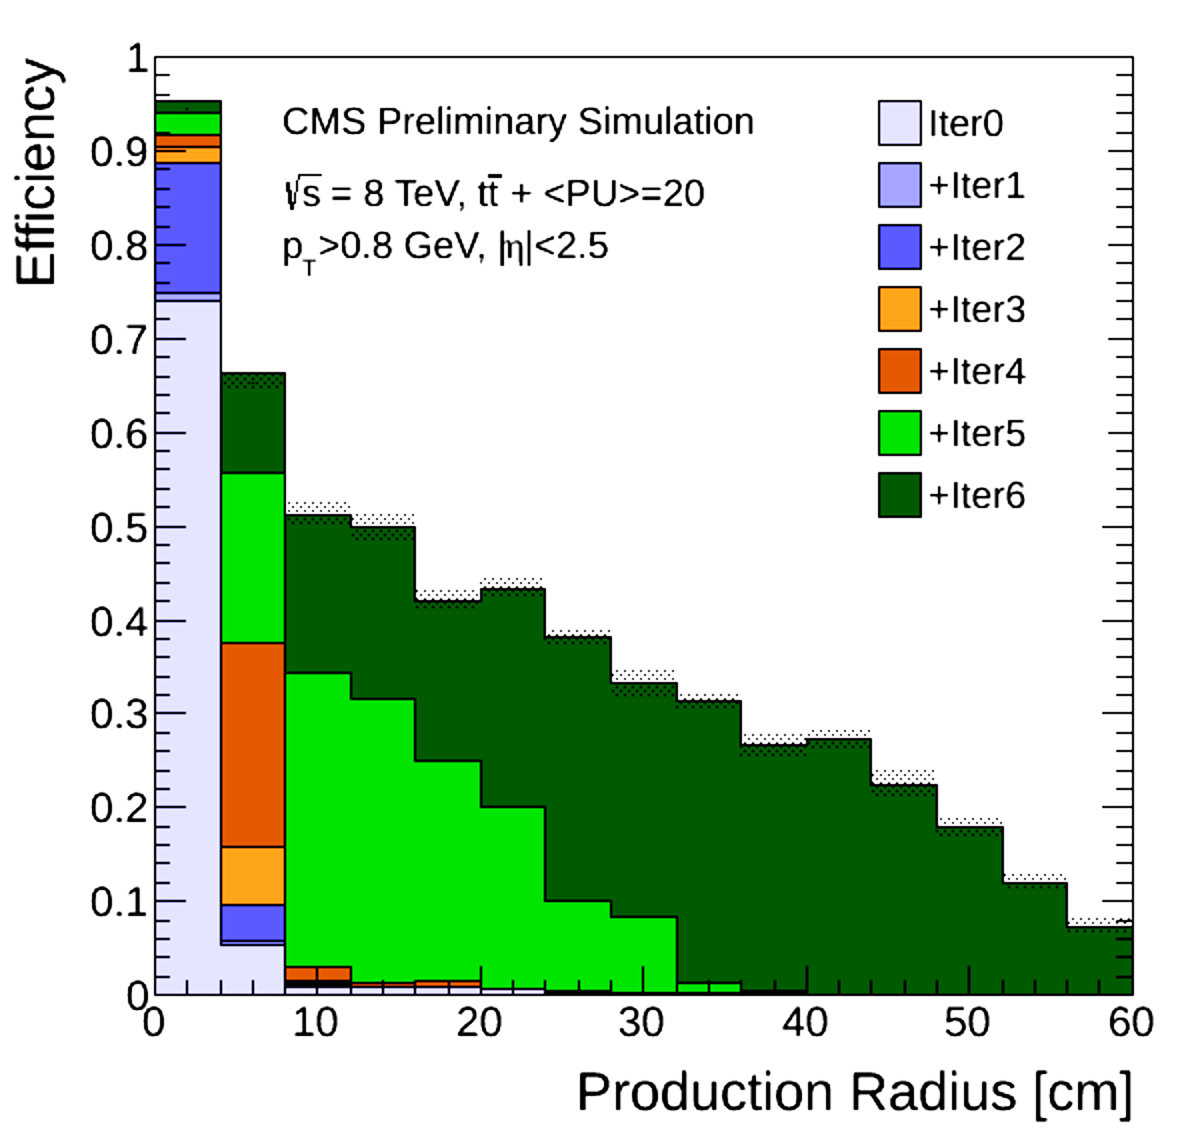
\includegraphics[width=0.45\textwidth]{figures/reconstruction/tracking_vs_vertpos.jpg}
}

%##############################################
\section{Particle flow}
%##############################################

%##############################################
\section{Muons}
%##############################################

%##############################################
\section{Electrons}
%##############################################

%##############################################
\section{Jets}
%##############################################

CHS, JEC, JER

%##############################################
\section{b-tagging}
%##############################################

SF, rizzi recipe

%##############################################
\section{Missing transverse energy}
%##############################################

T0, T1 corrections

%##############################################
\section{Luminosity and pileup}
%##############################################

pileup, rho
